\documentclass[aspectratio=1610]{beamer}
%\documentclass[aspectratio=1610, handout]{beamer}
\usepackage[utf8]{inputenc}
\usepackage{ragged2e}
\usepackage{xcolor}
\usepackage[italian]{babel}
\usepackage{multirow}
\usetheme[progressbar=frametitle,titleformat=smallcaps]{metropolis}
\setbeamertemplate{frame numbering}[fraction]
\setbeamercovered{dynamic}
\definecolor{rosso}{RGB}{255, 0, 0}
\definecolor{giallo}{RGB}{254,212,23}
\hypersetup{colorlinks=true,linkcolor=black,urlcolor=rosso}
\setbeamercolor{palette primary}{fg=black, bg=giallo}
\setbeamercolor{background canvas}{bg=white}
\setbeamercolor{normal text}{fg=black}
\setbeamercolor{progress bar}{fg=rosso}
\setbeamercolor{framesubtitle}{fg=rosso}
\setbeamercolor{normal text .dimmed}{fg=giallo}
\setbeamercolor{block title alerted}{fg=rosso, bg=giallo}
\setbeamerfont{caption}{size=\tiny}
\setbeamerfont{caption name}{size=\tiny}
\setlength{\abovecaptionskip}{0pt}
\makeatletter
\metroset{block=fill}
\setlength{\metropolis@progressinheadfoot@linewidth}{1pt} 
\setlength{\metropolis@progressonsectionpage@linewidth}{1pt}
\setlength{\metropolis@titleseparator@linewidth}{1pt}
\makeatother

\title{INTERNET}
\subtitle{storia e struttura}
\date{}
\institute{\textit{
        Fonti:
        \begin{itemize}
            \item[-] \href{https://www.isoc.it/storia-di-internet}{Internet Society}
            \item[-] \href{https://www.fastweb.it/fastweb-plus/digital-magazine/storia-del-progetto-arpanet/}{Fastweb Plus}
            \item[-] \href{https://www.wired.it/internet/web/2019/03/11/internet-world-wide-web-storia/}{Wired}
            \item[-] \href{https://www.mozilla.org/it/firefox/browsers/browser-history/}{Mozilla}
        \end{itemize}
    }
}

\begin{document}

\begin{frame}[plain, noframenumbering]
    \titlepage
\end{frame}

\section{STORIA DI INTERNET}

\begin{frame}{1957: SPUTNIK}
    \begin{alertblock}{FATTORE SCATENANTE}
        \begin{minipage}{0.98\linewidth}
            \justifying
            \textbf{1957}: L'unione sovietica manda in orbita il primo satellite artificiale intorno alla Terra, vincendo la 
            sfida spaziale contro gli Stati Uniti durante il periodo della Guerra Fredda.\\
            \textbf{\textit{``In the eyes of the world, first in space means first, period. Second in space is 
            second in everything."}}\\
            Lyndon Johnson, 1957\\
            \bigskip
            \tiny{\textbf{Video}}\\
            \tiny{\href{https://www.youtube.com/watch?v=xSQpBUkwyPo}{Sputnik Terrified Americans (David Hoffman)}}
        \end{minipage}
    \end{alertblock}
\end{frame}

\begin{frame}{1969: ARPANET}
    \begin{columns}
        \column{.4\textwidth}
            \begin{alertblock}{CREAZIONE DI ARPANET}
                \begin{minipage}{0.98\linewidth}
                    \justifying
                    \textbf{1969}: Il progenitore e precursore della rete Internet è considerato il progetto \textbf{ARPANET}, finanziato dalla 
                    DARPA (Defence Advanced Research Projects Agency) un'agenzia dipendente dal Ministero della Difesa statunitense.\\
                \end{minipage}
            \end{alertblock}
        \column{.5\textwidth}
            \begin{figure}
                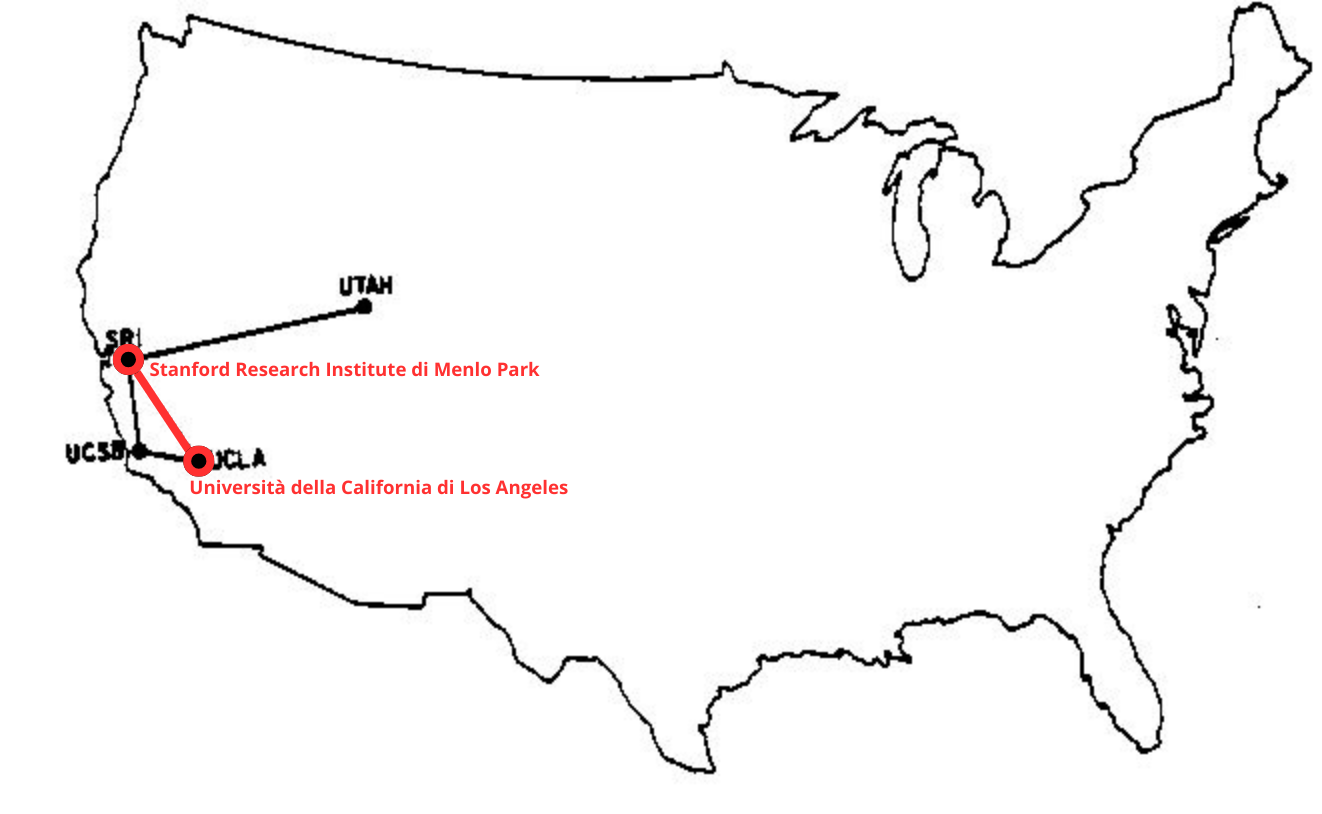
\includegraphics[width=\linewidth]{img/arpanet.png}
                \caption{{Fonte \href{http://mercury.lcs.mit.edu/~jnc/tech/arpageo.html}{ARPANET Maps}}}
            \end{figure}
    \end{columns}
\end{frame}

\begin{frame}{1991: WORLD WIDE WEB}
    \begin{alertblock}{CREAZIONE DEL WWW}
        \begin{minipage}{0.98\linewidth}
            \justifying
            \textbf{1991}: Tim Berners-Lee, un ingegnere informatico britannico, inventa il \textbf{World Wide Web} (WWW), mette per 
            iscritto le tre tecnologie che sono le fondamenta del web: l’\textbf{HTML} (il linguaggio per la formattazione e 
            l’impaginazione di documenti ipertestuali), la \textbf{URL} (l’indirizzo unico che permette di identificare ogni singola 
            risorsa presente in rete) e il protocollo \textbf{HTTP} che permette di recuperare tutte le risorse linkate.\\
            \bigskip
            \tiny{\textbf{Curiosità}}\\
            \tiny{\href{https://www.w3.org/History/1989/proposal.html}{Tim Berners-Lee: A Proposal}}
        \end{minipage}
    \end{alertblock}
\end{frame}

\begin{frame}{1993: BROWSER}
    \begin{alertblock}{CREAZIONE DI MOSAIC}
        \begin{minipage}{0.98\linewidth}
            \justifying
            \textbf{1993}: \textbf{Mosaic} venne creato presso il National Center for Supercomputing Applications (NCSA), 
            nell’Università dell’Illinois Urbana-Champaign, dall’informatico Marc Andreessen. Si tratta del primo 
            browser web popolare e il primo antenato di Mozilla Firefox.\\
            \bigskip
            \tiny{\textbf{Curiosità}}\\
            \tiny{\href{https://en.m.wikipedia.org/wiki/Killer\_application}{Mosaic Killer}}
        \end{minipage}
    \end{alertblock}
\end{frame}

\begin{frame}{INTERNET OGGI}
    \begin{figure}
        \href{https://www.geopop.it/storia-della-nascita-di-internet-come-lo-usiamo-oggi-e-come-funziona-il-world-wide-web/}{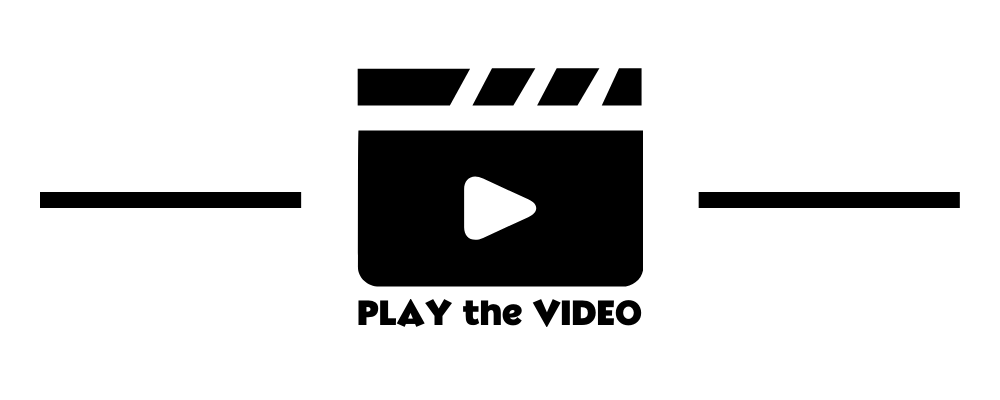
\includegraphics[width=\linewidth]{img/play.png}}
        \caption{{Fonte \href{https://www.geopop.it/storia-della-nascita-di-internet-come-lo-usiamo-oggi-e-come-funziona-il-world-wide-web/}{La storia di Internet (Geopop)}}}
    \end{figure}
    \bigskip
    \tiny{\textbf{Curiosità}}\\
    \tiny{\href{https://attivissimo.blogspot.com/2022/01/hacker-nel-far-west.html}{Hacker nel Far West}} 
\end{frame}

\section{STRUTTURA DI INTERNET}

\begin{frame}{STRUTTURA DI INTERNET}
    \only<1 | handout:0>{\begin{figure}
        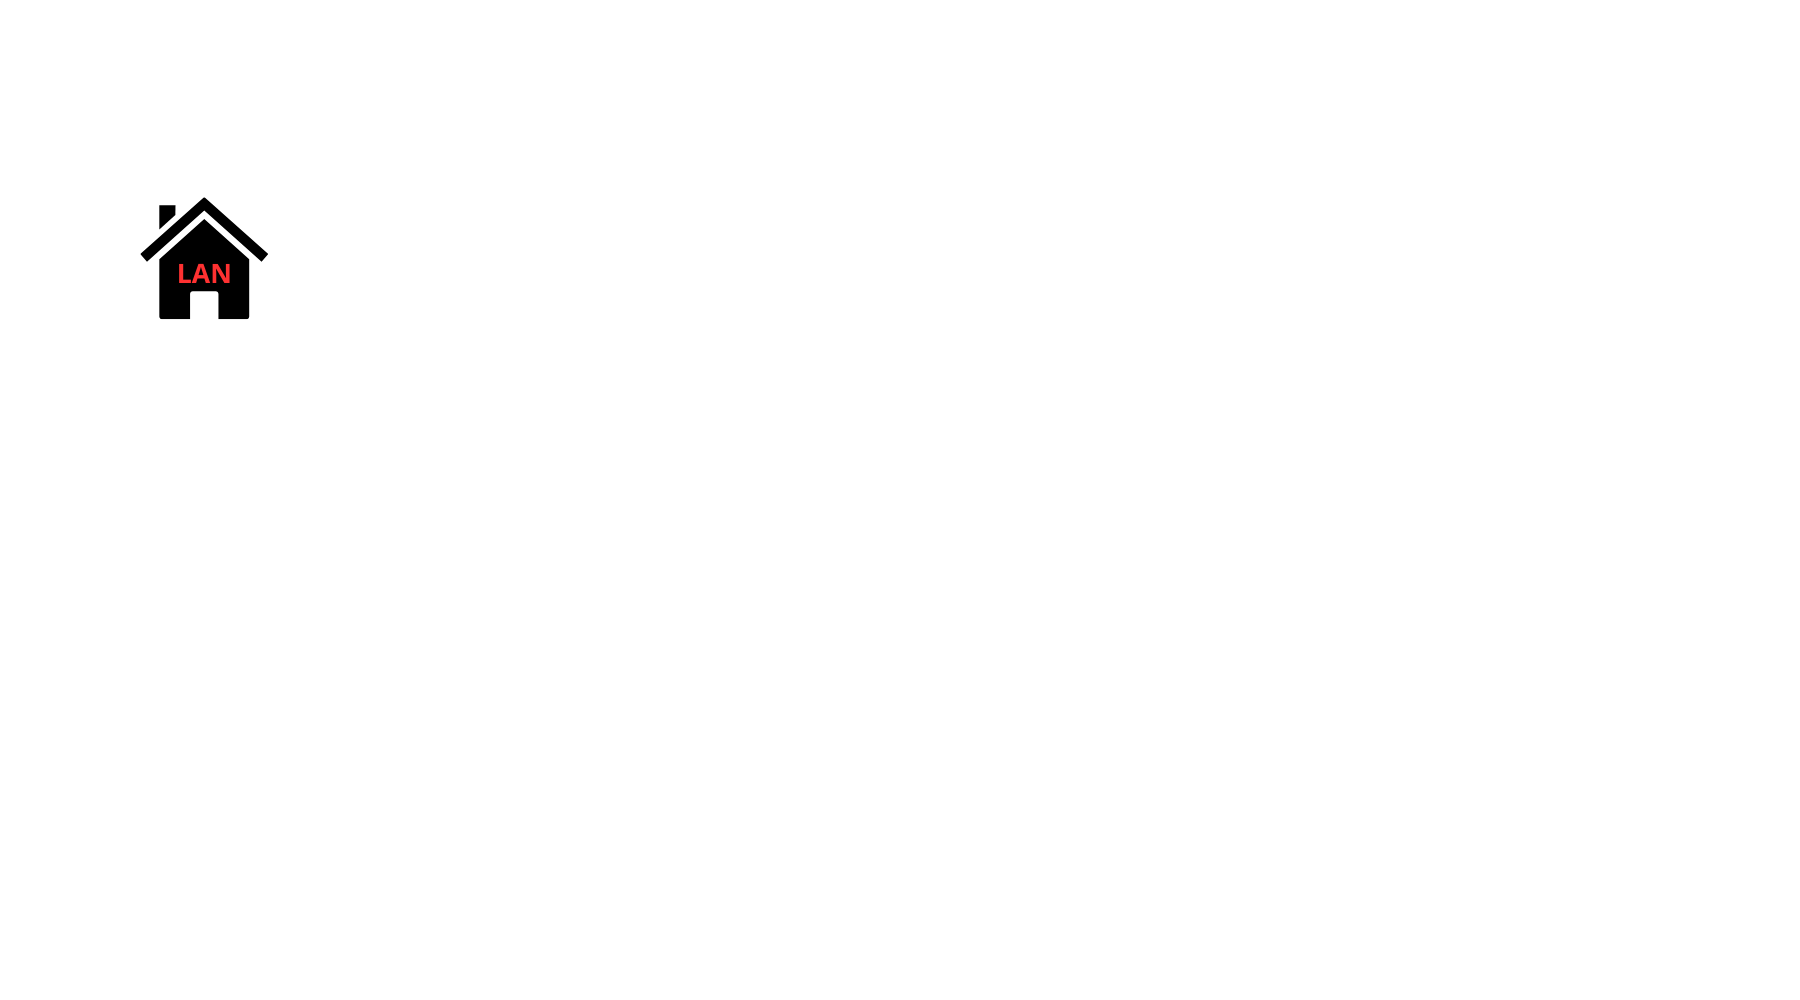
\includegraphics[width=\linewidth]{img/internet1.png}
        \caption{{creata con \href{https://www.canva.com/}{Canva}}}
    \end{figure}}
    \only<2 | handout:0>{\begin{figure}
        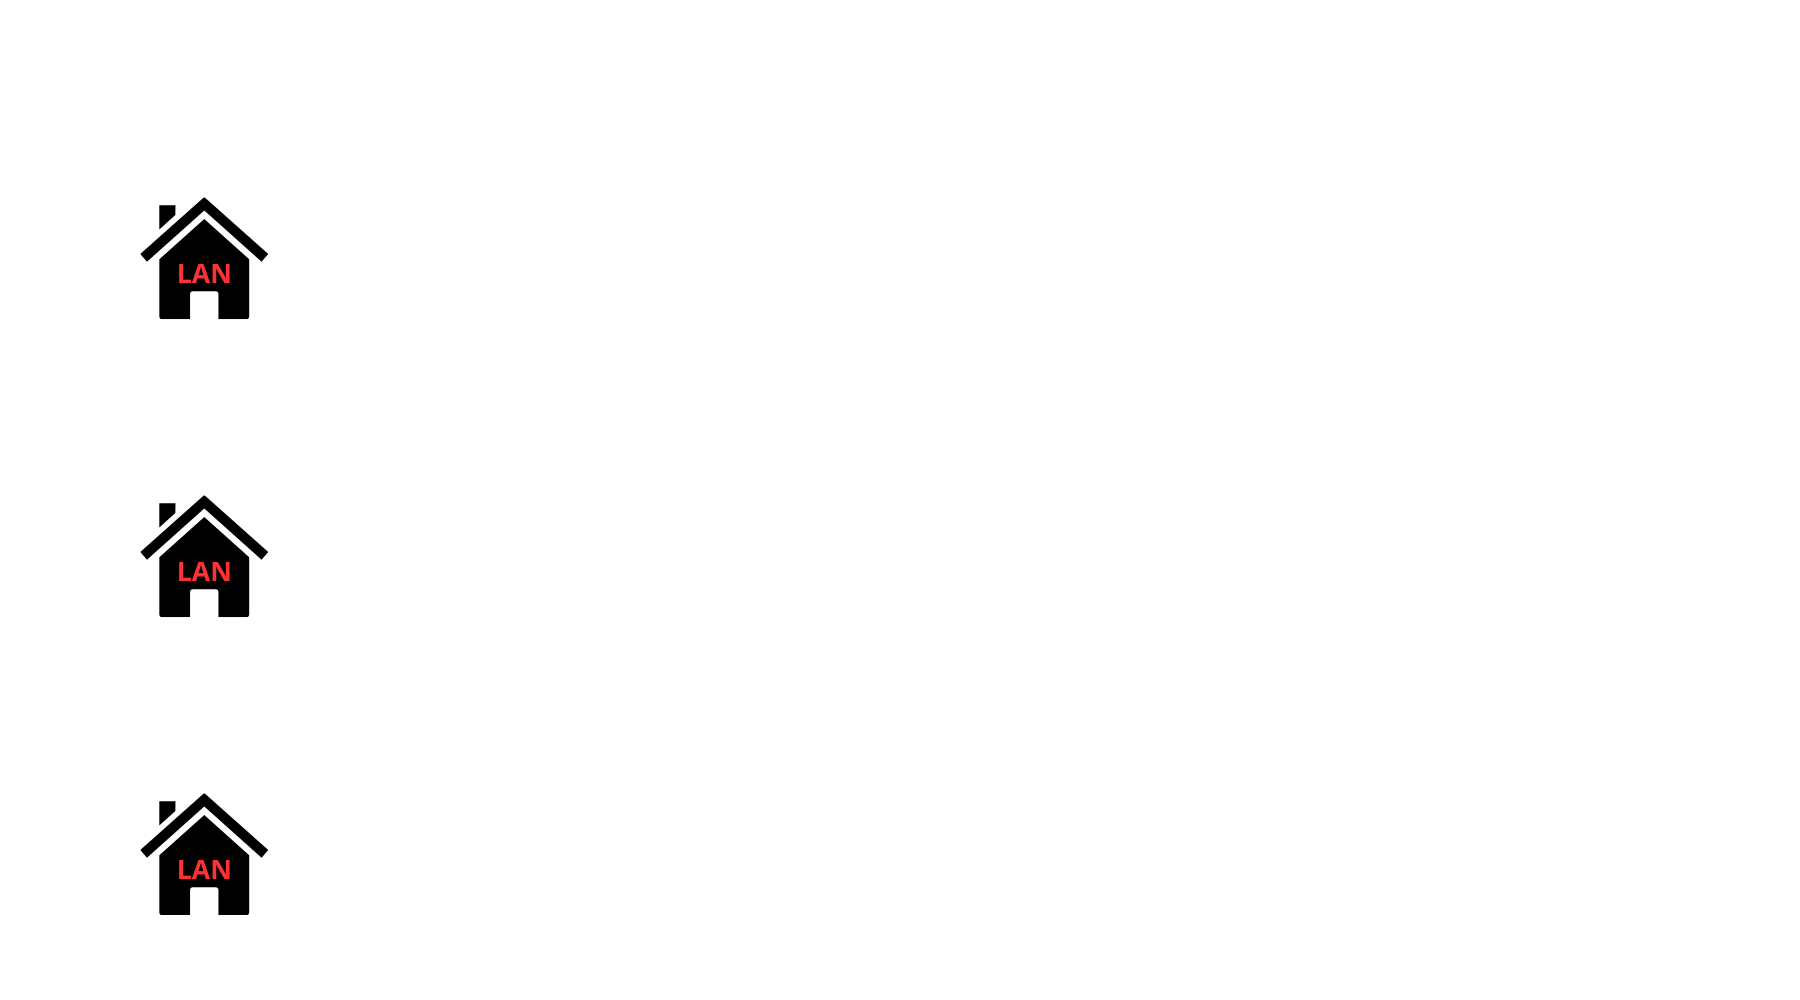
\includegraphics[width=\linewidth]{img/internet2.png}
        \caption{{creata con \href{https://www.canva.com/}{Canva}}}
    \end{figure}}
    \only<3 | handout:0>{\begin{figure}
        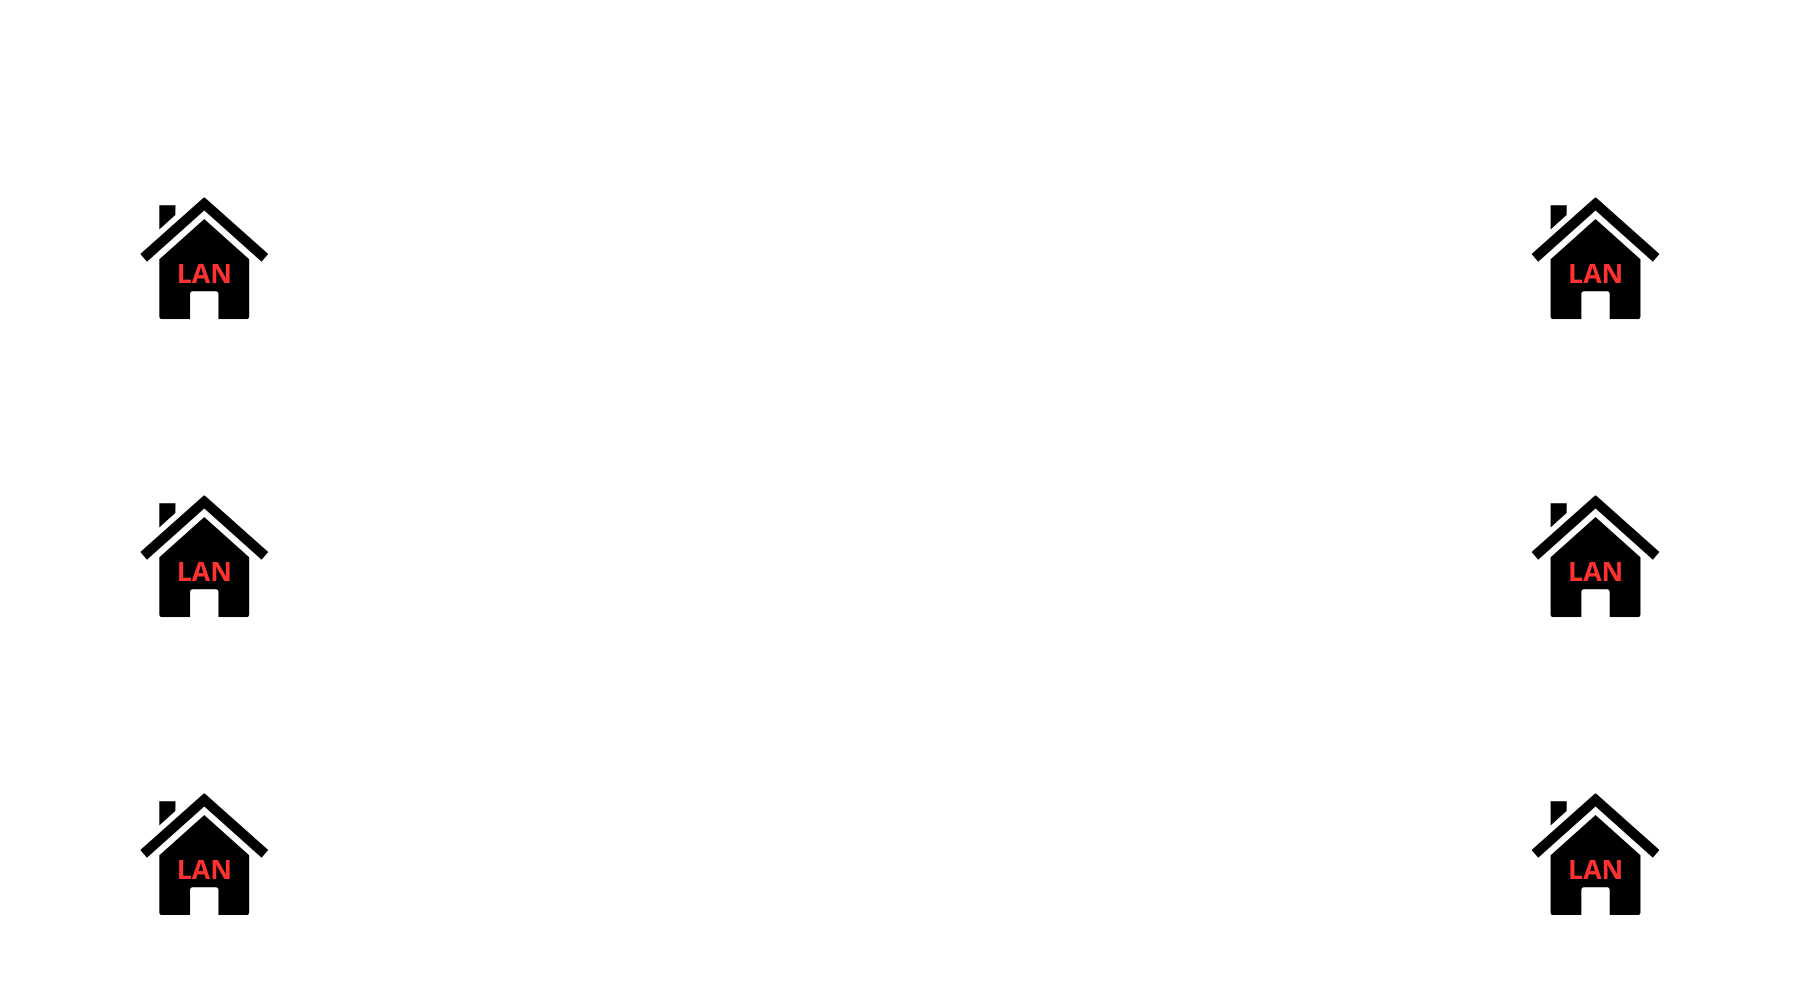
\includegraphics[width=\linewidth]{img/internet3.png}
        \caption{{creata con \href{https://www.canva.com/}{Canva}}}
    \end{figure}}
    \only<4 | handout:1>{\begin{figure}
        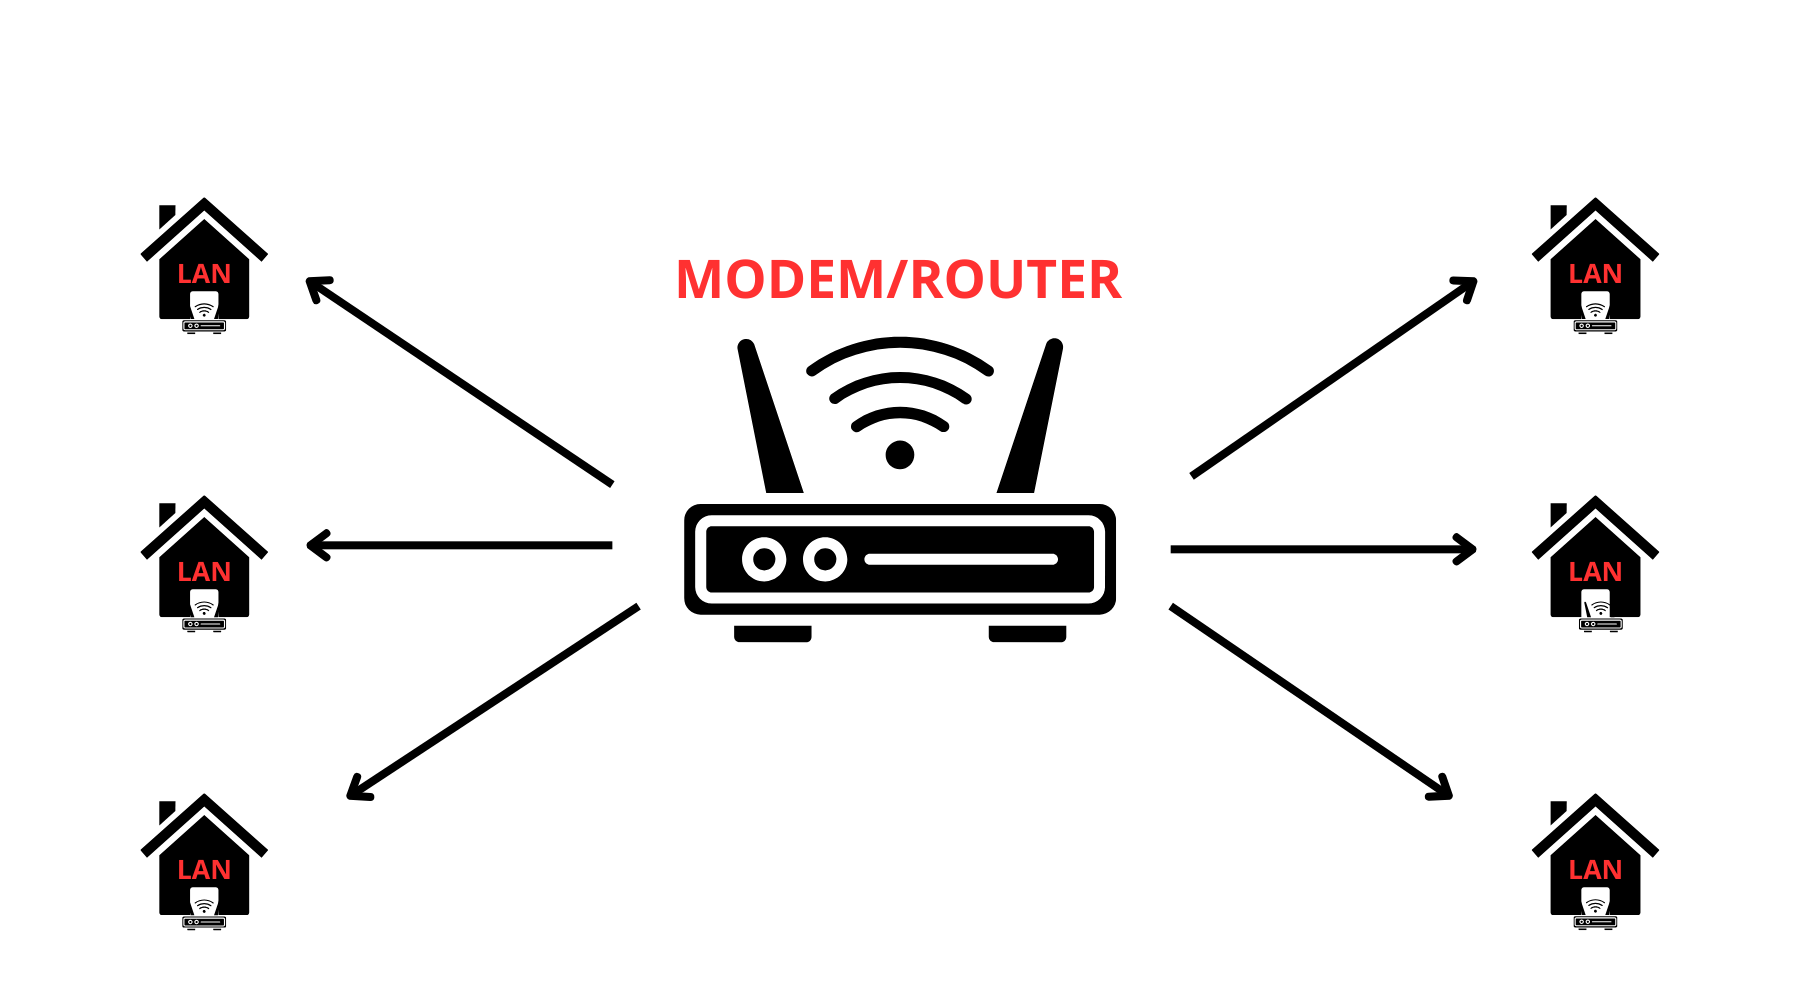
\includegraphics[width=\linewidth]{img/internet4.png}
        \caption{{creata con \href{https://www.canva.com/}{Canva}}}
    \end{figure}}
    \only<5 | handout:0>{\begin{figure}
        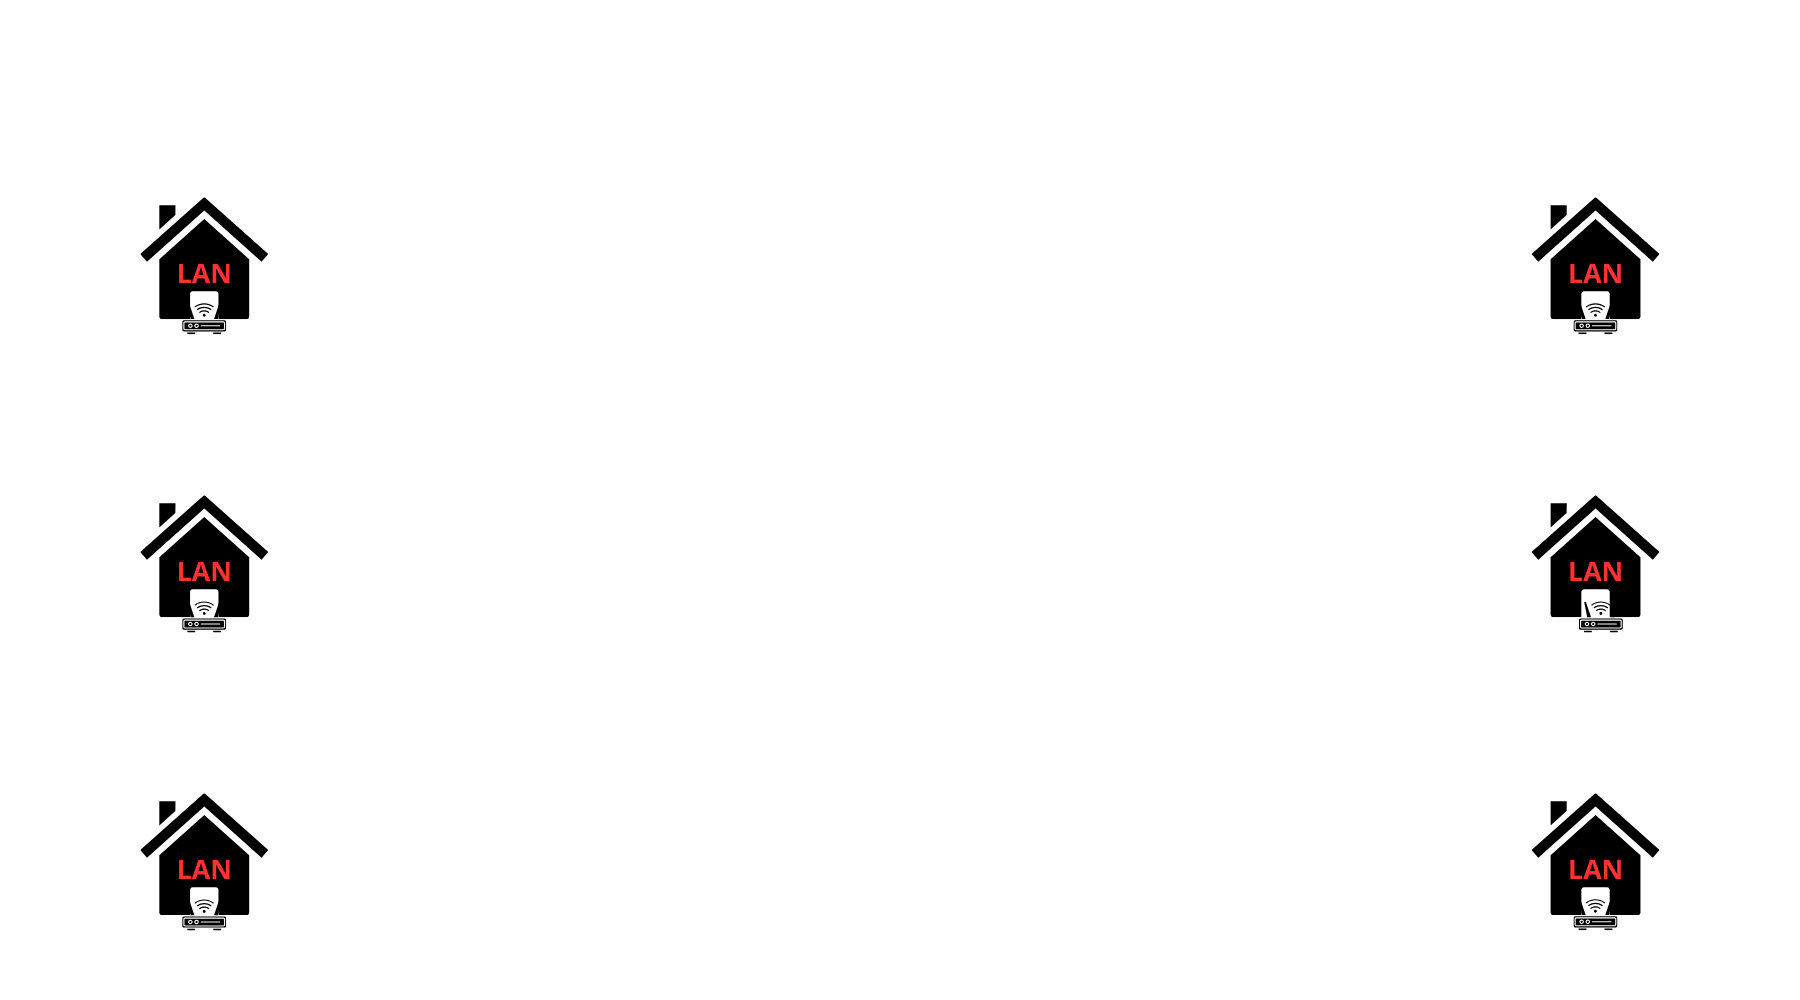
\includegraphics[width=\linewidth]{img/internet5.png}
        \caption{{creata con \href{https://www.canva.com/}{Canva}}}
    \end{figure}}
    \only<6 | handout:2>{\begin{figure}
        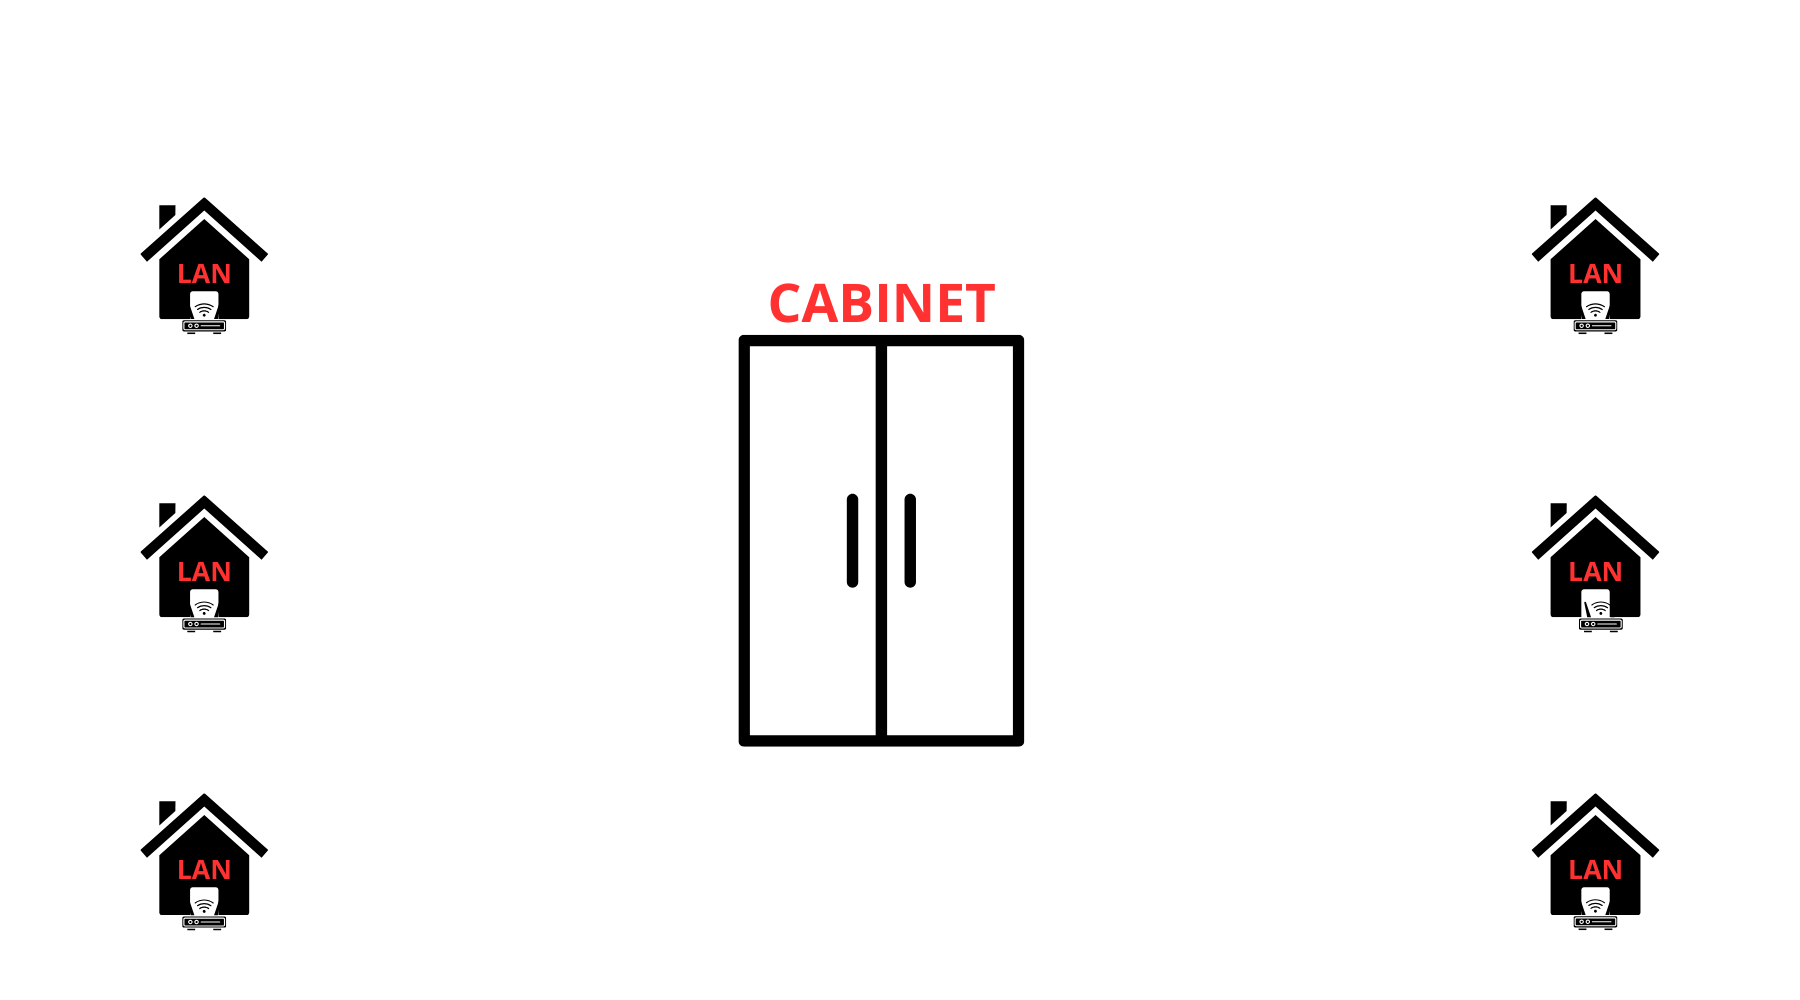
\includegraphics[width=\linewidth]{img/internet6.png}
        \caption{{creata con \href{https://www.canva.com/}{Canva}}}
    \end{figure}}
    \only<7 | handout:0>{\begin{figure}
        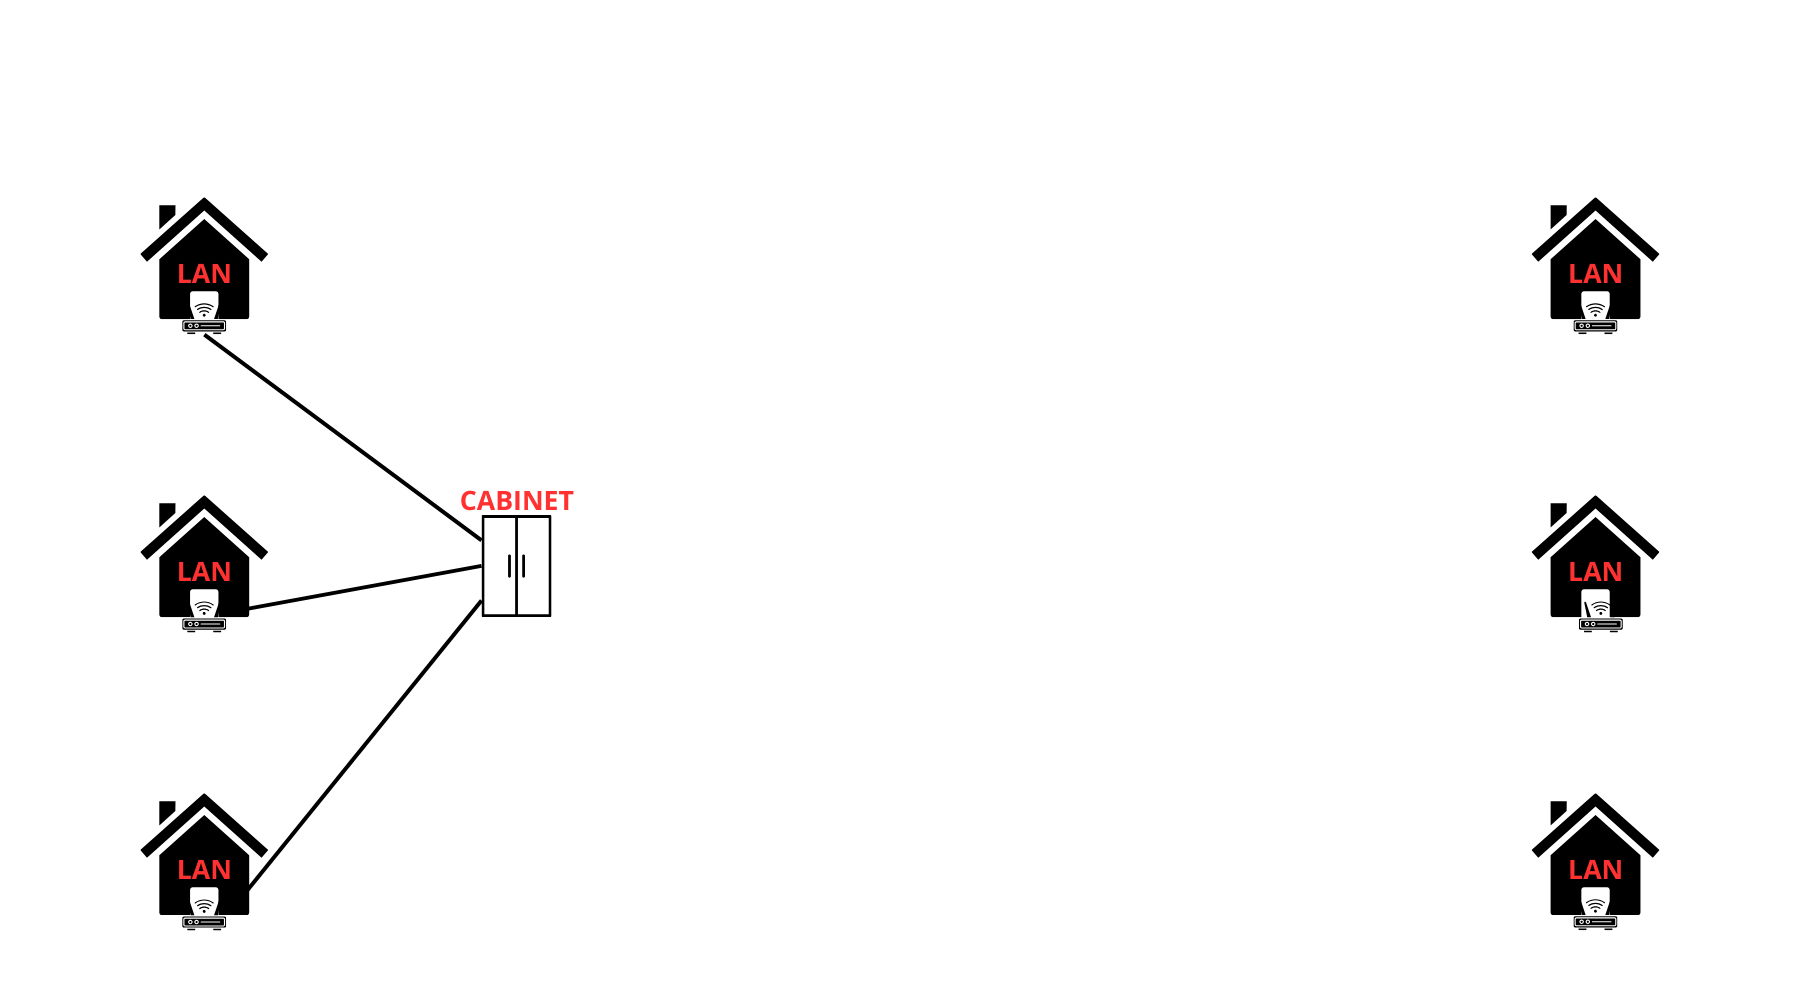
\includegraphics[width=\linewidth]{img/internet7.png}
        \caption{{creata con \href{https://www.canva.com/}{Canva}}}
    \end{figure}}
    \only<8 | handout:0>{\begin{figure}
        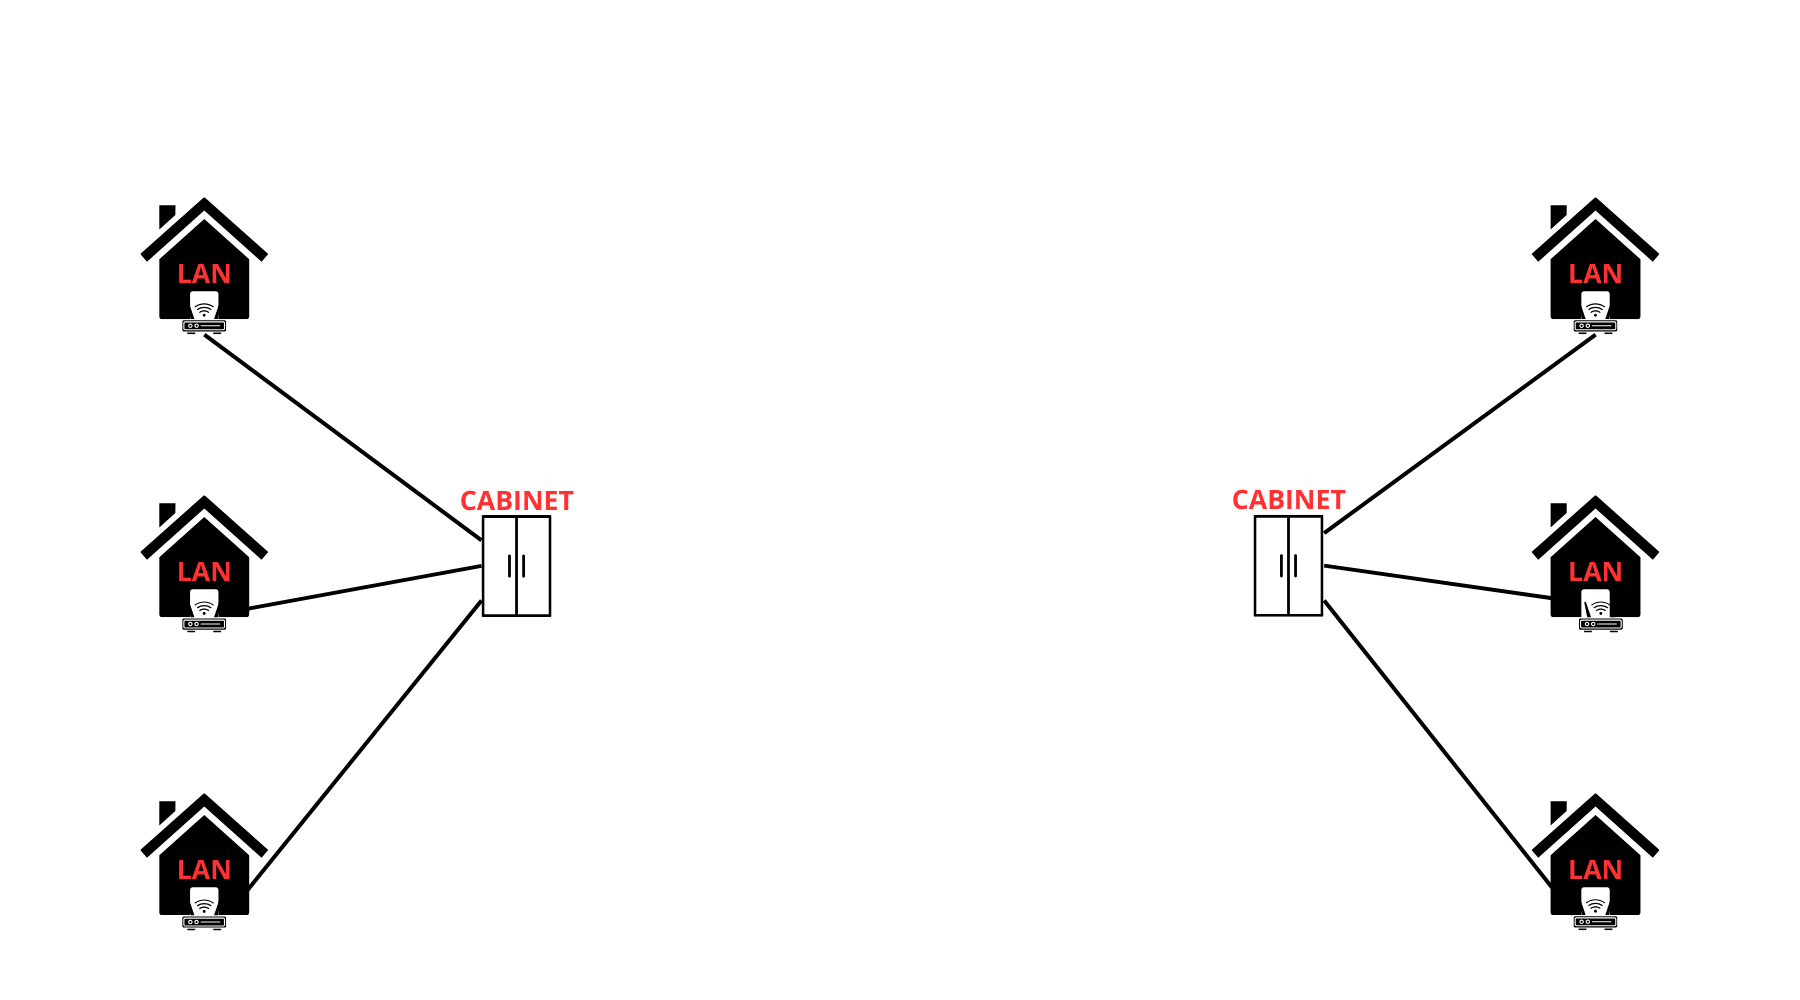
\includegraphics[width=\linewidth]{img/internet8.png}
        \caption{{creata con \href{https://www.canva.com/}{Canva}}}
    \end{figure}}
    \only<9 | handout:0>{\begin{figure}
        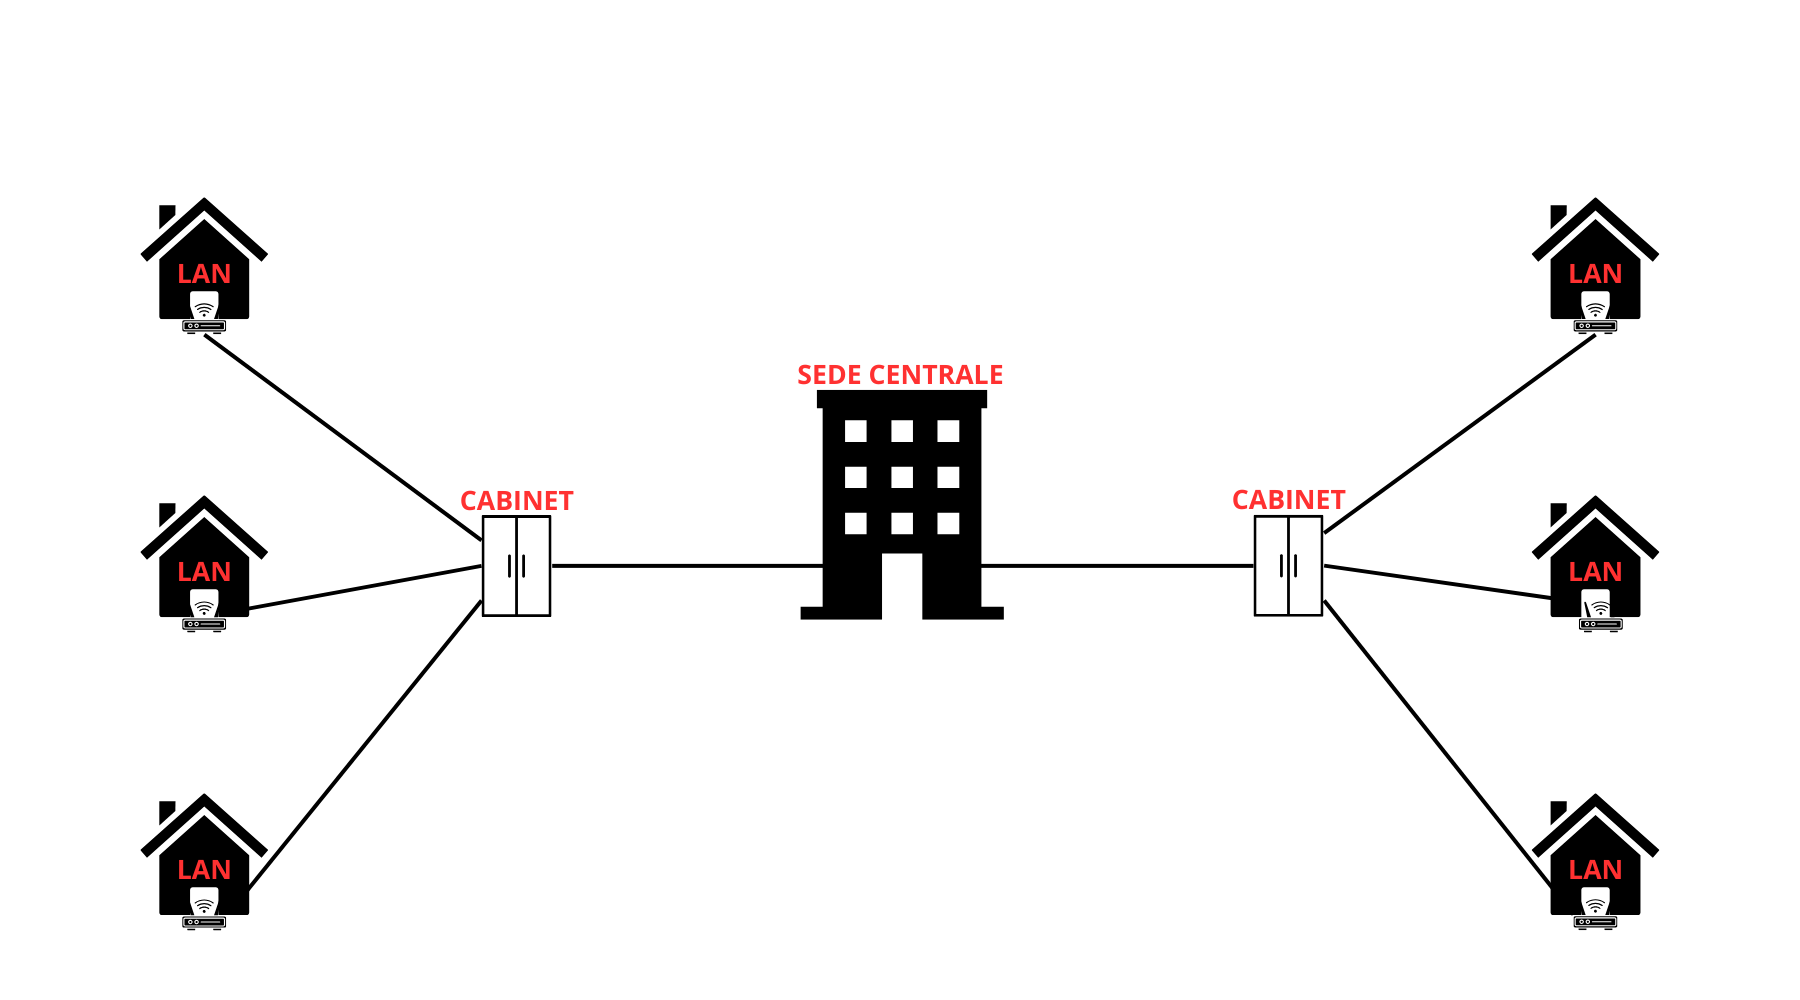
\includegraphics[width=\linewidth]{img/internet9.png}
        \caption{{creata con \href{https://www.canva.com/}{Canva}}}
    \end{figure}}
    \only<10 | handout:3>{\begin{figure}
        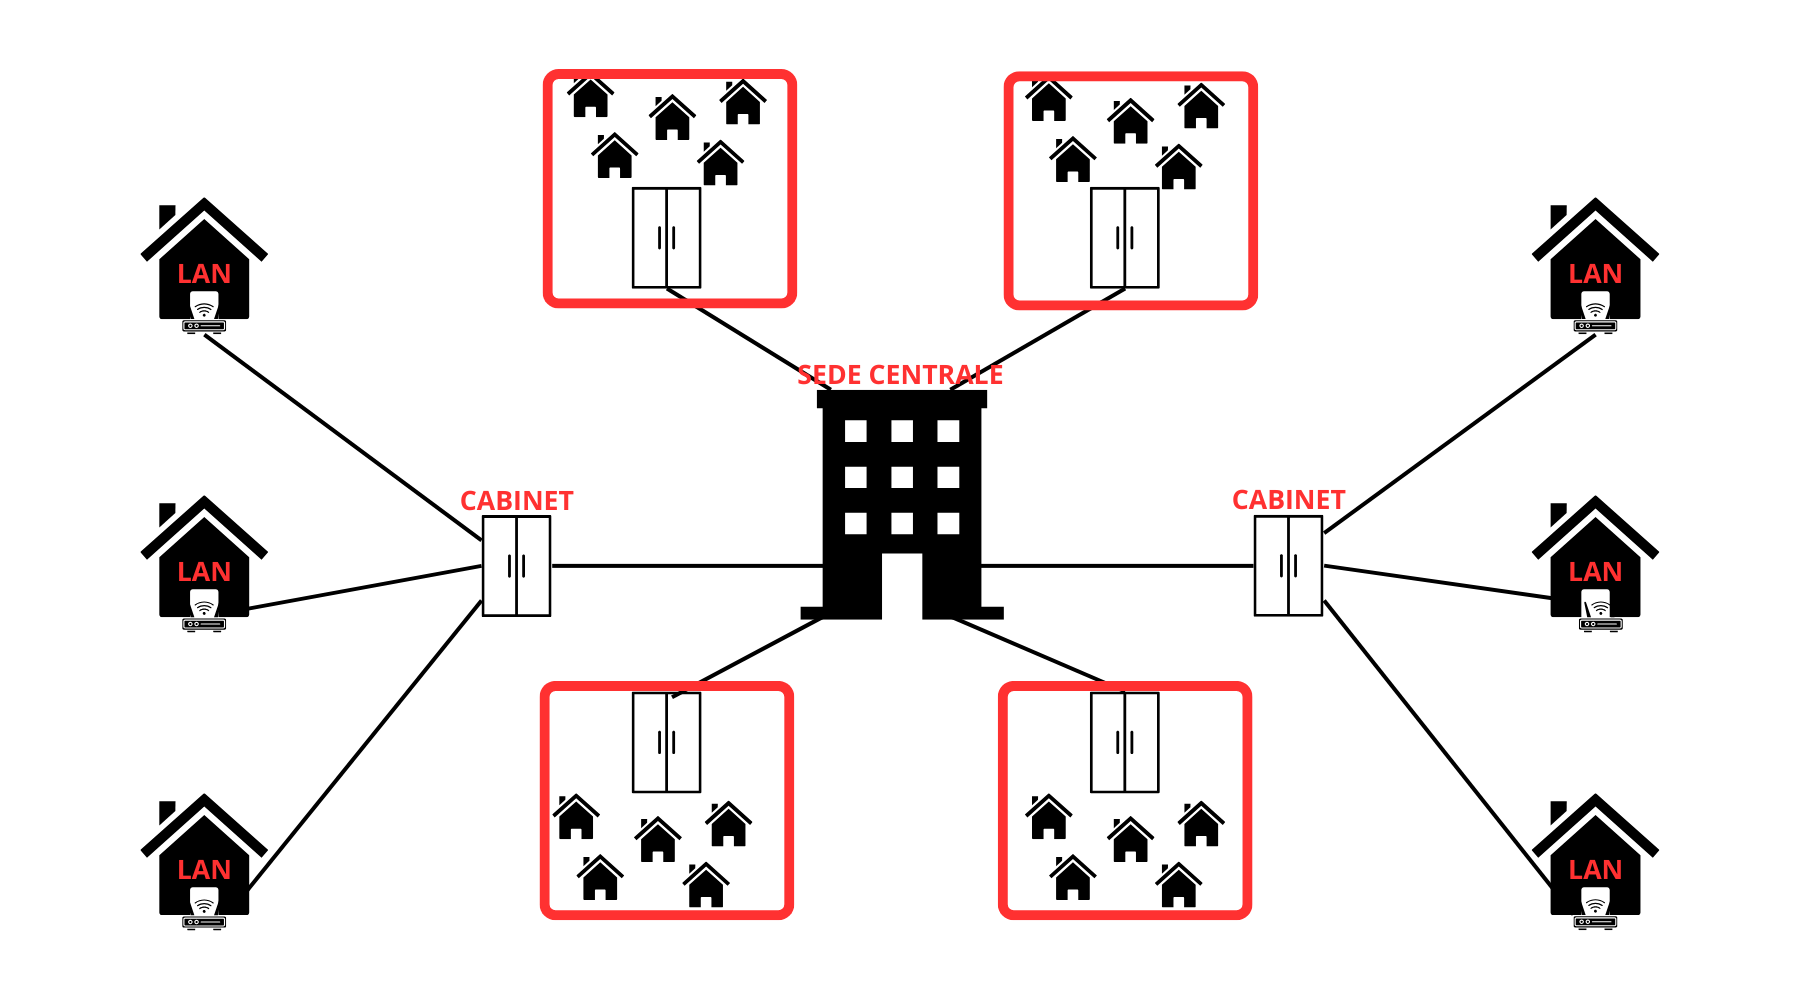
\includegraphics[width=\linewidth]{img/internet10.png}
        \caption{{creata con \href{https://www.canva.com/}{Canva}}}
    \end{figure}}
    \only<11 | handout:0>{\begin{figure}
        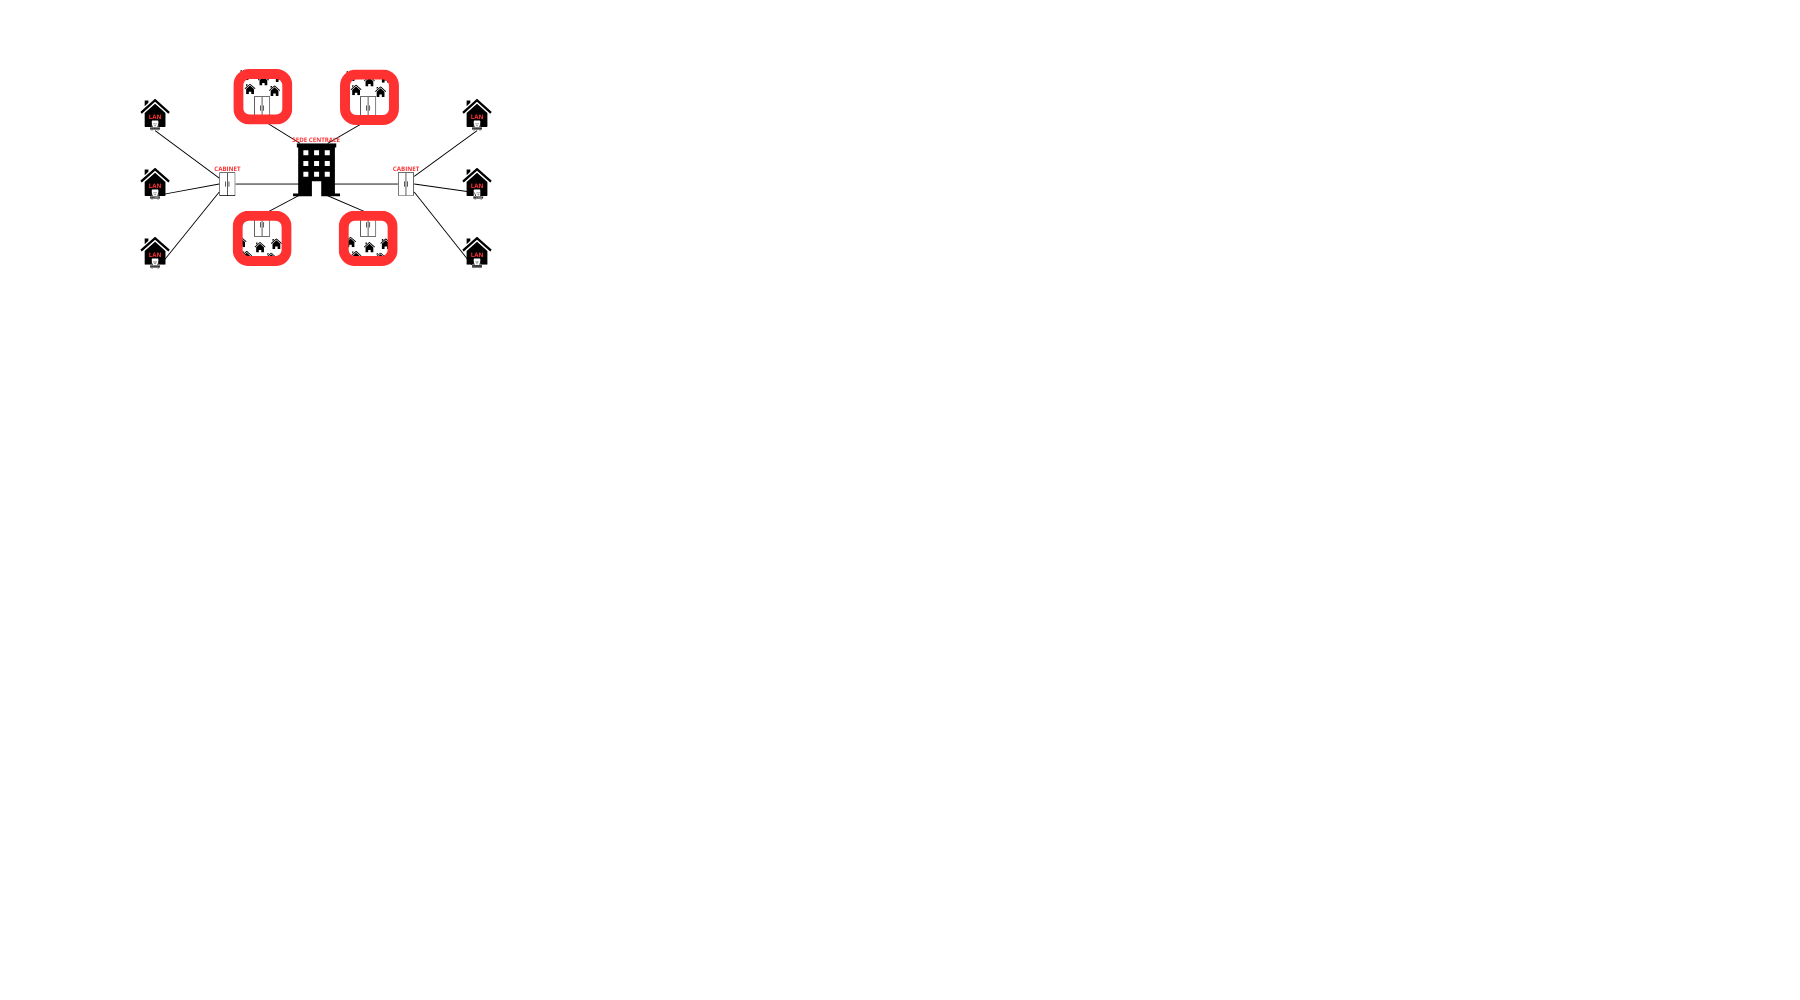
\includegraphics[width=\linewidth]{img/internet11.png}
        \caption{{creata con \href{https://www.canva.com/}{Canva}}}
    \end{figure}}
    \only<12 | handout:0>{\begin{figure}
        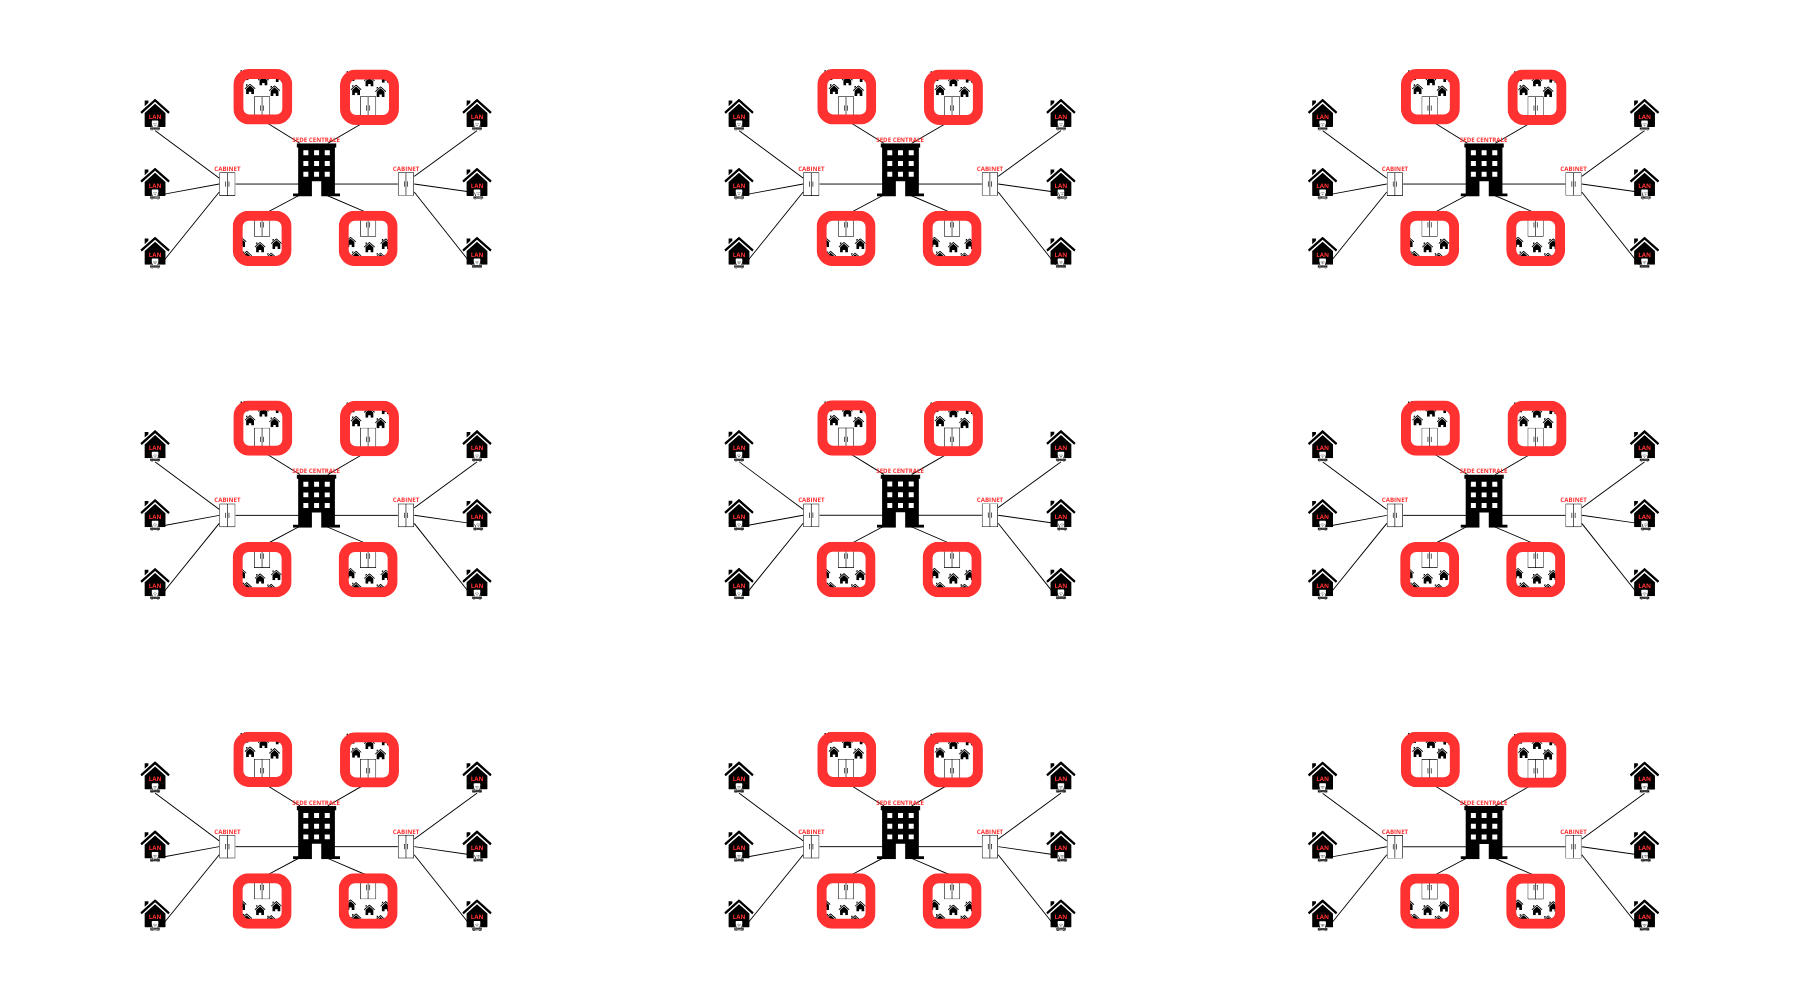
\includegraphics[width=\linewidth]{img/internet12.png}
        \caption{{creata con \href{https://www.canva.com/}{Canva}}}
    \end{figure}}
    \only<13 | handout:4>{\begin{figure}
        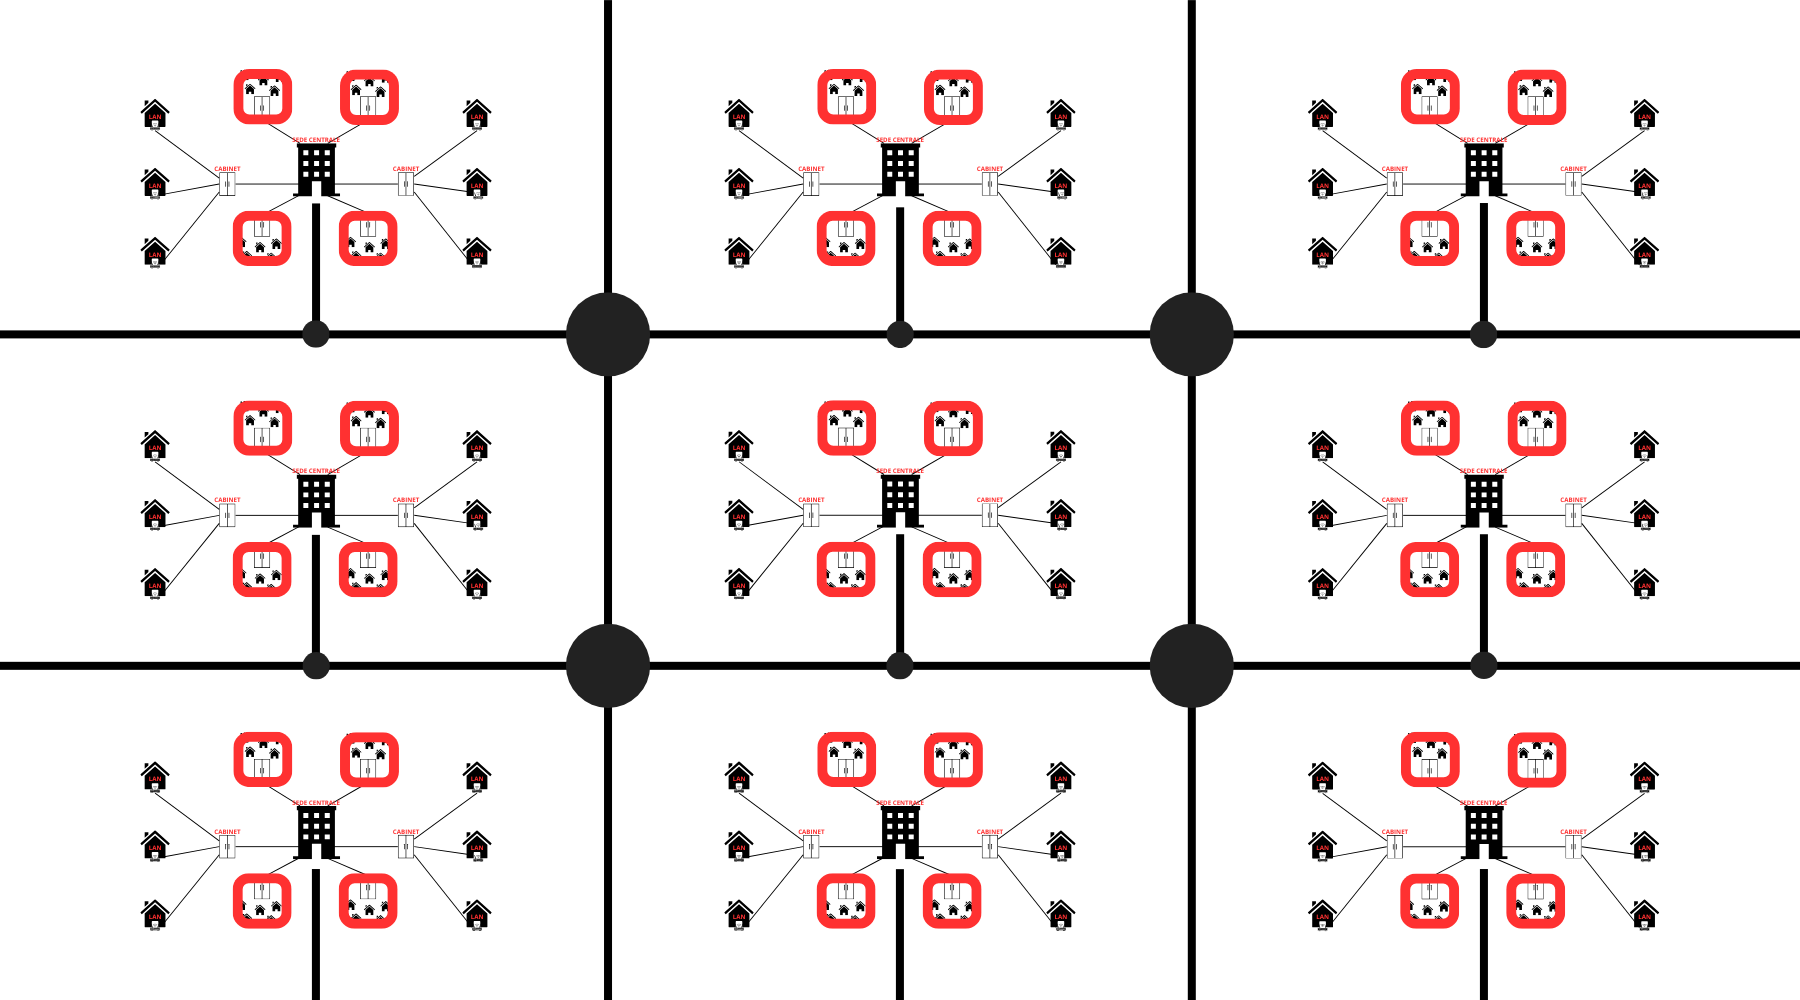
\includegraphics[width=\linewidth]{img/internet13.png}
        \caption{{creata con \href{https://www.canva.com/}{Canva}}}
    \end{figure}}
    \only<14 | handout:0>{\begin{figure}
        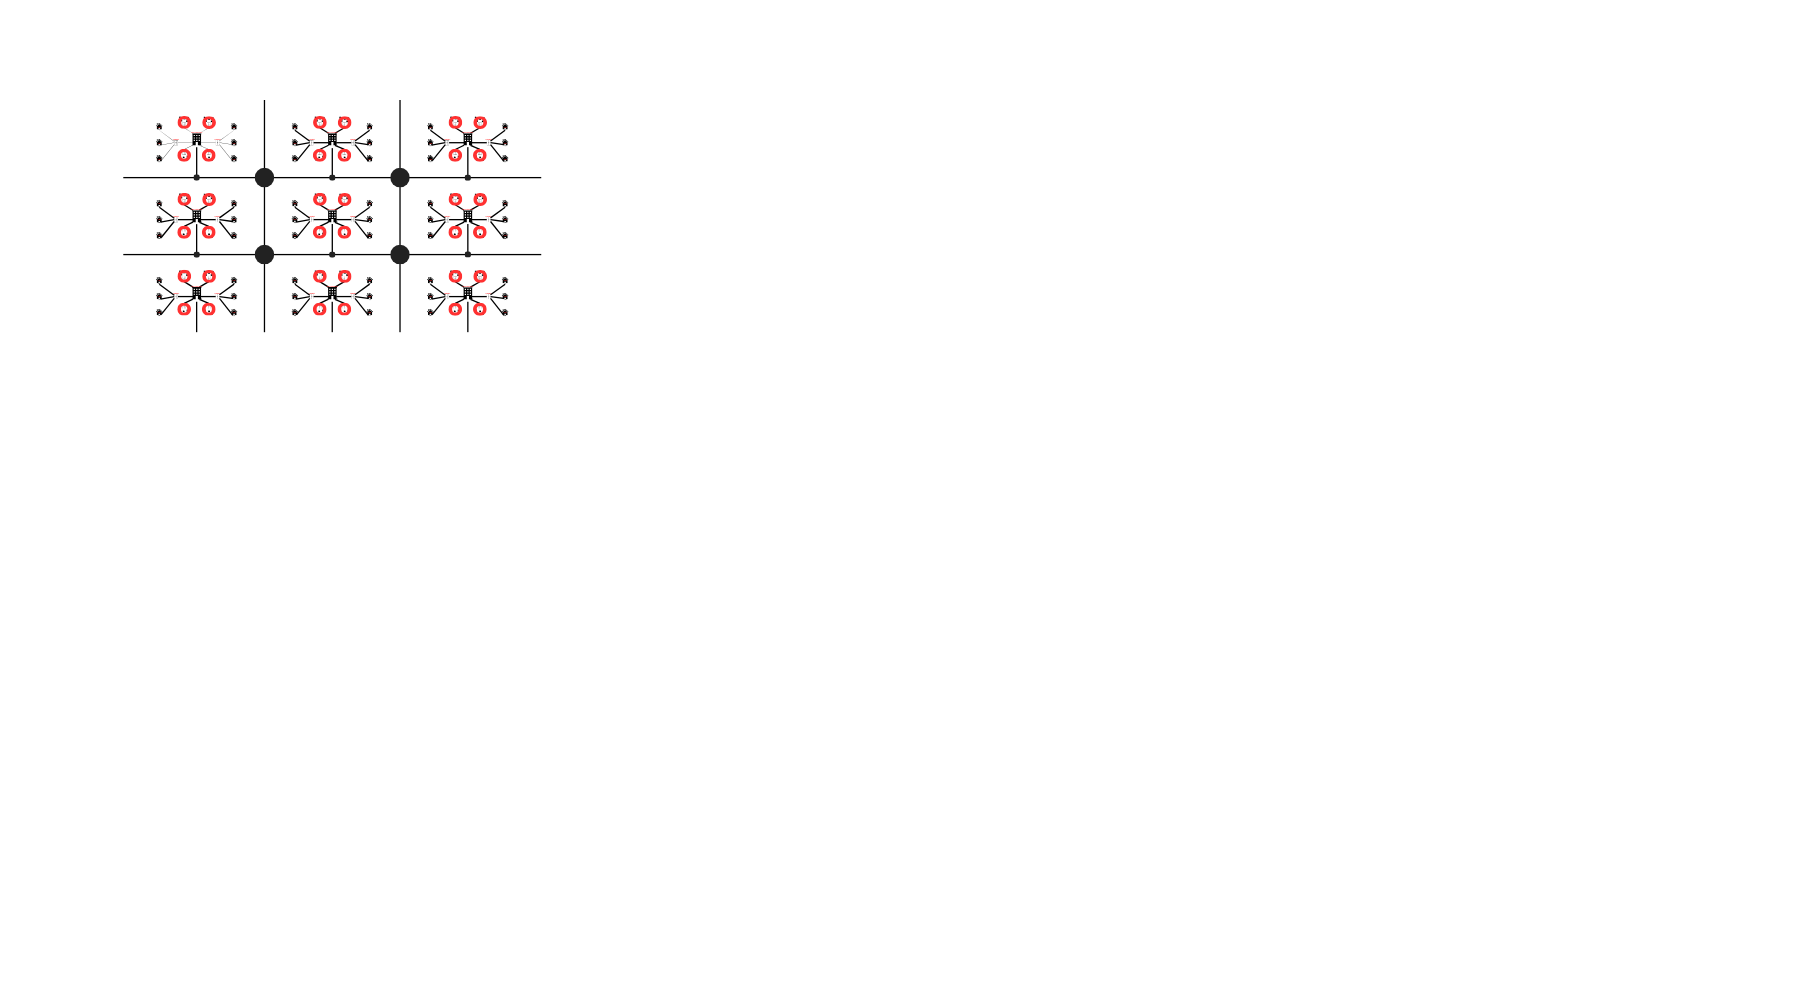
\includegraphics[width=\linewidth]{img/internet14.png}
        \caption{{creata con \href{https://www.canva.com/}{Canva}}}
    \end{figure}}
    \only<15 | handout:5>{\begin{figure}
        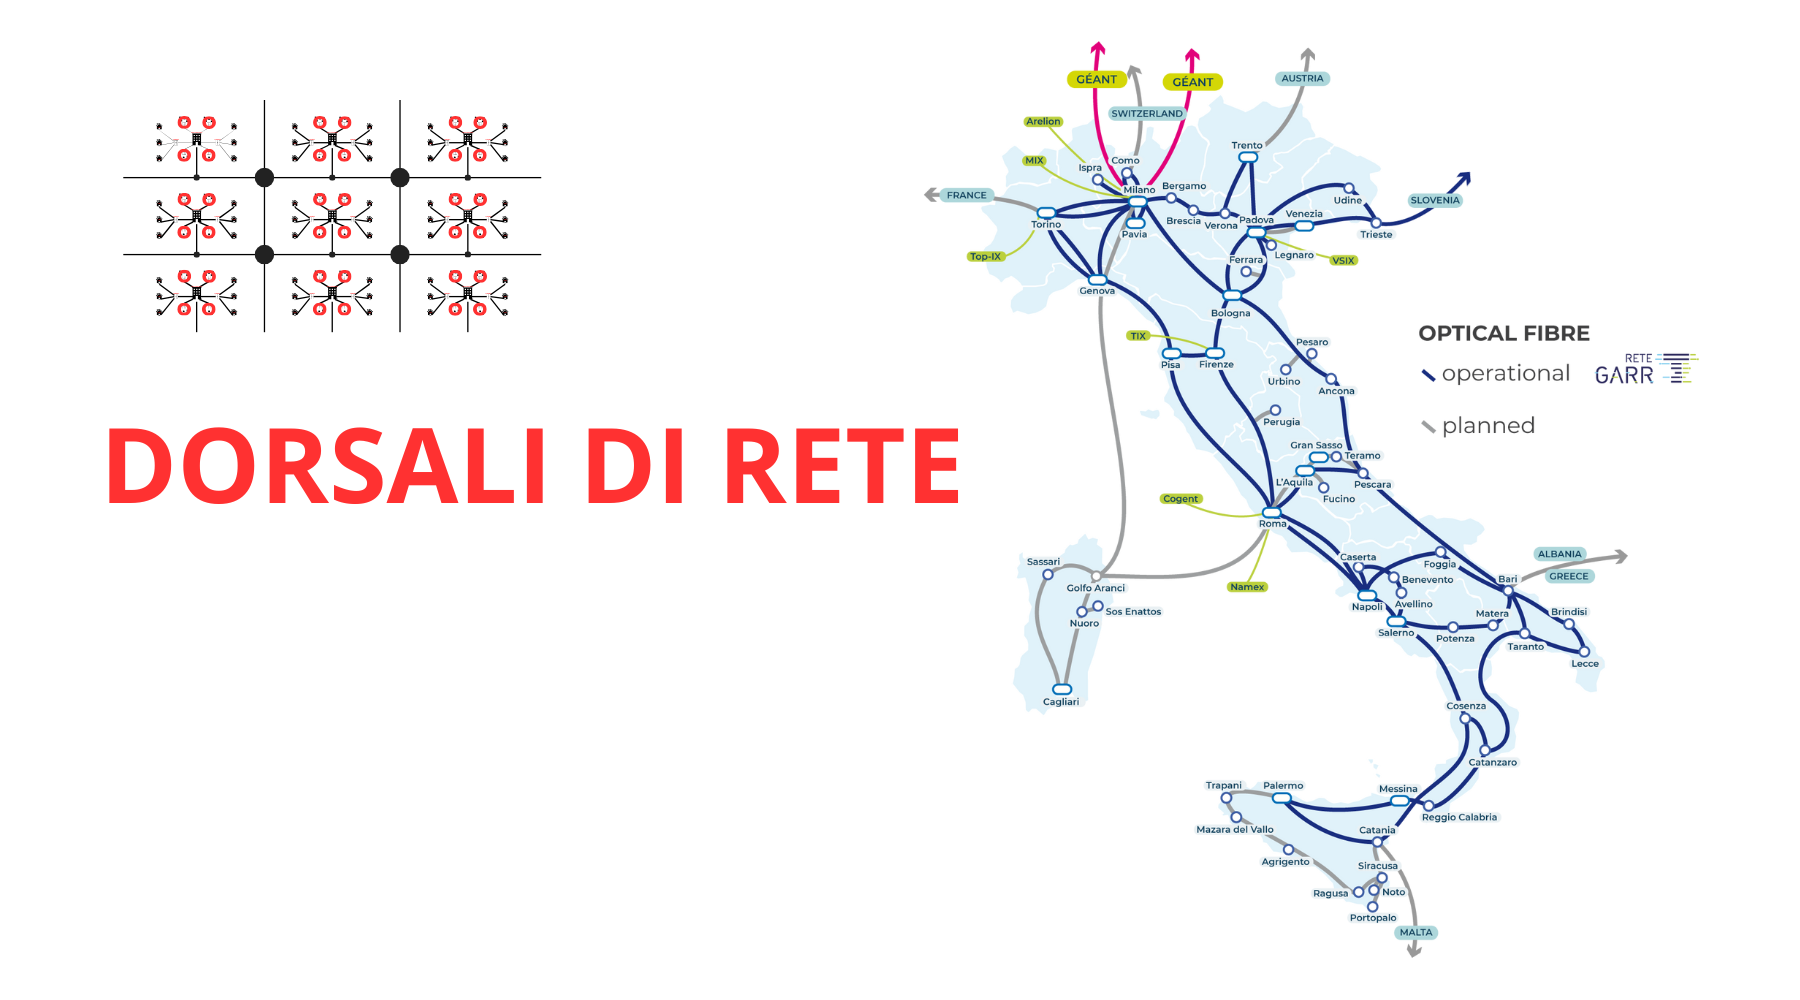
\includegraphics[width=\linewidth]{img/internet15.png}
        \caption{{creata con \href{https://www.canva.com/}{Canva}, Fonte \href{https://www.garr.it/it/infrastrutture/rete-nazionale/mappa-della-rete}{GARR}}}
    \end{figure}}
\end{frame}

\begin{frame}{SUBMARINE CABLE MAP}
    \begin{figure}
        \href{https://www.submarinecablemap.com/}{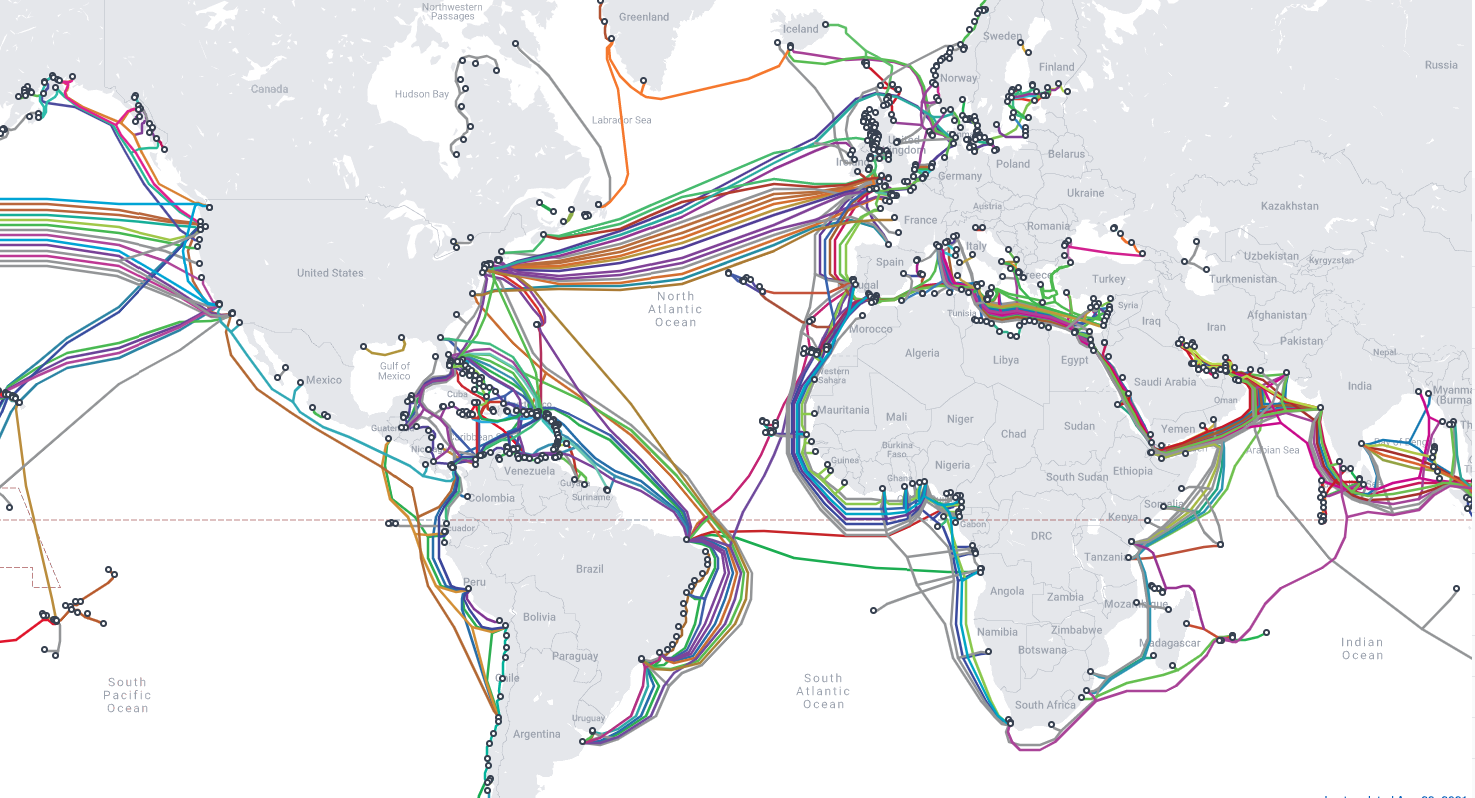
\includegraphics[width=.8\linewidth]{img/SubmarineCableMap.png}}
        \caption{{Fonte \href{https://www.submarinecablemap.com/}{Submarine Cable Map}}}
    \end{figure}       
    \bigskip
    \tiny{\textbf{Curiosità}}\\
    \tiny{\href{https://blog.telegeography.com/topic/maps}{Mappe Telegeography}} 
\end{frame}

\begin{frame}{CAVI SOTTOMARINI}
    \begin{figure}
        \href{https://www.geopop.it/serie/cavi-sottomarini/}{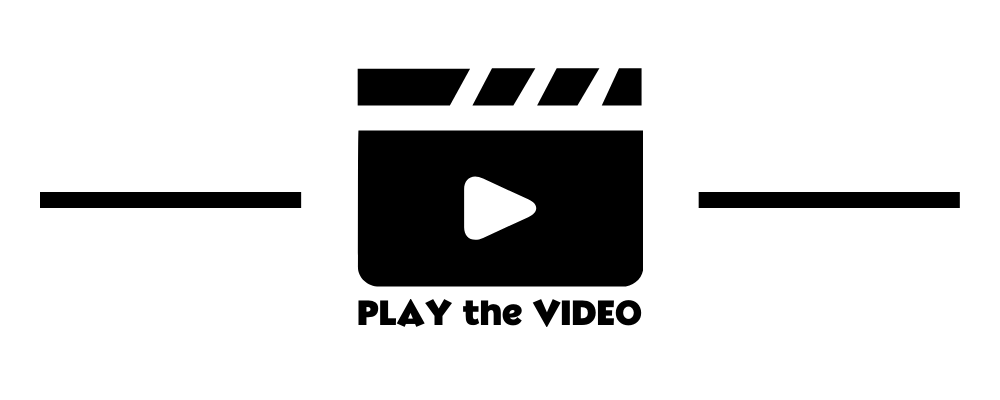
\includegraphics[width=\linewidth]{img/play.png}}
        \caption{{Fonte \href{https://www.geopop.it/serie/cavi-sottomarini/}{Cavi sottomarini (Geopop)}}}
    \end{figure}   
    \bigskip
    \tiny{\textbf{Curiosità}}\\
    \tiny{
        \href{https://www.cybersecurity360.it/cybersecurity-nazionale/lera-di-splinternet-cosi-la-geopolitica-sta-fratturando-il-cyberspazio/}{Splinternet} e 
        \href{https://www.agendadigitale.eu/infrastrutture/cavi-tranciati-a-suez-goretti-namex-ecco-come-ridurre-il-rischio/}{cavi tranciati canale di Suez}\\
        \href{https://techcrunch.com/2024/11/29/meta-plans-to-build-a-10b-subsea-cable-spanning-the-world-sources-say/}{Meta's "W" cable}
    }     
\end{frame}

\begin{frame}{STRUTTURA RETE MOBILE}
    \begin{figure}
        \href{https://www.geopop.it/il-percorso-del-segnale-del-telefono-quando-chiamiamo-o-inviamo-messaggi/}{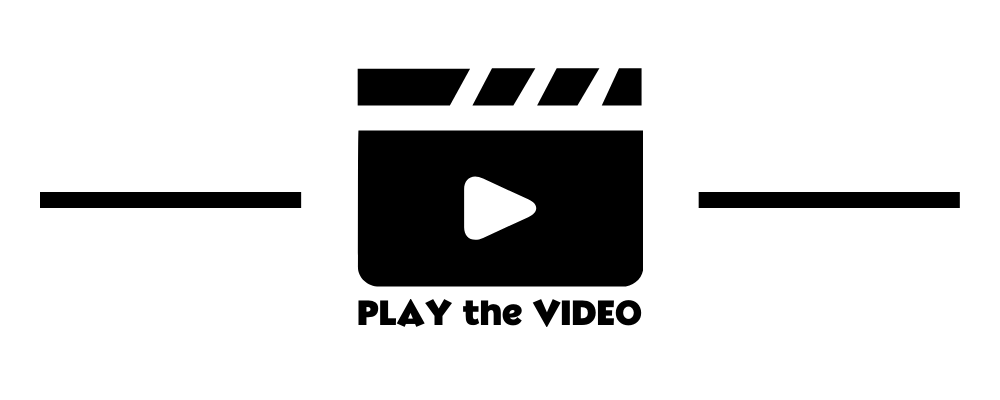
\includegraphics[width=\linewidth]{img/play.png}}
        \caption{{Fonte \href{https://www.geopop.it/il-percorso-del-segnale-del-telefono-quando-chiamiamo-o-inviamo-messaggi/}{Il viaggio del segnale (Geopop)}}}
    \end{figure}        
    \bigskip
    \tiny{\textbf{Curiosità}}\\
    \tiny{
        \href{https://geo.agcom.it/agcomapps/BB4/BB4_BBmobile_app17_1/}{Mappa rete mobile}\\
        \href{https://www.geopop.it/5g-vs-4g-quali-sono-le-differenze-e-i-vantaggi-della-nuova-generazione/}{4G vs 5G}
    } 
\end{frame}

\end{document}